\documentclass[pdftex,10pt,a4paper,twocolumn]{article}
\title{\textbf{Developing a cellular automaton model for kidney morphogenesis}}
\author{Ben Lambert}
\usepackage[titletoc,toc]{appendix}
\usepackage[pdftex]{graphicx}
\usepackage{url,times}
\usepackage{graphicx}
\usepackage{epstopdf}
\usepackage{amsmath}
\usepackage[all]{xy}
\usepackage{pxfonts}
\usepackage{colortbl}
\usepackage{color}
\usepackage{subfigure}
\usepackage{gensymb}
\usepackage{ctable}
\usepackage[justification=centering]{caption}[2007/12/23]
\usepackage{longtable}
\usepackage{pst-func}
\usepackage{pst-math}
\renewcommand{\bibname}{Works Cited}
\usepackage{listings}
\usepackage{setspace}
\usepackage{algorithm}
\usepackage{bbm}



\newcommand{\HRule}{\rule{\linewidth}{0.5mm}}
\begin{document}

\twocolumn[
\maketitle
\doublespacing
\begin{@twocolumnfalse}
\begin{abstract}
\textbf{Kidney development involves interactions between two distinct populations of cells: the metanephric mesenchyme and the epithelium of the Wolffian Duct. From 10.5-11 days post egg fertilisation (stages E10-11.5 in mouse organ cultures) a uretic bud (UB) of epithelium forms, which invades the space of the mesenchyme; later undergoing branching and extension which ultimately results in the components of a functioning kidney: the nephrons and collecting duct. In this paper a simple cellular automaton model is presented which recapitulates the initial emergence of the UB, along with its primary branching. In the model, mesenchymal cells release a diffusible growth factor GDNF, which binds to Ret receptors on epithelial cells, influencing their behaviour. The model is then used to make predictions relating the number of epithelial cells in the uretic bud to the initial number of mesenchymal cells; which may be able to be tested experimentally.}
\end{abstract}
\end{@twocolumnfalse}
]

\section{Introduction}
The human kidney's primary function is to filter blood of waste products (mainly urea) from metabolism. The most important functional units of a kidney are nephrons, which are responsible for regulating the concentration of water and other solutes released in urine. In a nephron blood is filtered by the Glomerulus, and the filtrate then flows through a system of structures (the proximal tubule, loop of Henle and the distal tubule), where filtrates are selectively reabsorbed, then connects with a collecting duct which delivers the waste products to the ureter for excretion.

A fully developed human kidney is composed of 200,000 to 1.8 million nephrons, connected by a system of collecting ducts to the ureter, with the majority of the structure being formed during the embryonic stages of life ~\cite{hughson2003glomerular}. There are functional consequences for reduced nephron number, with evidence suggesting that this can cause hypertension and renal failure in adult life ~\cite{hoy2008nephron}. Furthermore, kidney and urinary tract congenital disorders are amongst the most common birth defects ~\cite{airik2007down}, with hypoplasia and dysplasia occurring in up to 1/200 births \cite{weber2006prevalence}. These are suggestive that biological and computational models which can help illuminate the cause, action and potential remedy of these types of disorder would be of clinical value.

Experimental work has focussed on animal models (mice, rats and fish) to study renal development. Broadly, there are two categories of experiment which have been undertaken: \textit{in vivo} studies of the effects of knock-out genes, and \textit{in vitro} studies of explanted kidney cells, grown in particular culture media (containing GDNF as well as other factors). In particular, mouse studies have already demonstrated their relevance to the study of human kidneys. Dominant renal hypodysplastic kidneys, characteristic of a number of human renal disorders, display mutations in genes which were first discovered in the mouse ~\cite{LittleMMcMahon2012}.

During embryogenesis the early kidney is made up solely of undifferentiated cells, called the intermediate mesoderm (IM). These cells act as progenitors for all future nephron cells and collecting duct epithelium. At E9.5 in mouse studies the cells at the dorsal end of the organ form the epithelium of the Wolffian Duct extending in a rostro-caudal direction, with the rest of the cells maintaining their respective pluripotency ~\cite{CostantiniFKopan2010},\cite{saxen1987early}. Later on during development the remaining intermediate mesoderm becomes specialised along the rostro-caudal axis, with a relatively dense 'cloud' of mesenchyme forming at the caudal end ~\cite{CostantiniFKopan2010}, called the metanephric mesenchyme (MM).

In normal organ development at E10.5-11 (in mice), GDNF and other factors released by the MM, stimulate the outgrowth from the epithelium of a single discrete bud - the uretic bud (UB) - which invades the MM ~\cite{CostantiniFKopan2010},\cite{LittleMMcMahon2012}. The UB then undergoes rounds of branching and extension, resulting in the branched structure of the collecting duct and its associated tubules. During this time, there are a nexus of reciprocal interactions which determine the specific nature of the branched structure. 

The emergent bud, along with its branches are epithelial sheets with a central lumen, which may provide internal pressure to support the structure formed. It is important to note that, by contrast with epithelium in other branching morphologies, for example in vascular branching, the lumen is ever-present during development of the kidney \cite{Meyer2004}.

Factors produced by the epithelium also have a role to play in determining nephronic structure. In particular Wnt9b has been implicated in stimulating differentiation of mesenchymal cells proximal to the UB to form epithelium which acts as progenitors to nephrons. Normal development of the kidney's underlying structure stops at around parturition. Figure \ref{fig:real-branching} shows how branching of the initial uretic bud leads to the kidney structure.

Mathematical modelling of kidney development is still in its infancy. Branching of the uretic bud has been modelled with continuum PDE-based models, with mesenchyme cells producing GDNF, which in turn, via a cascade of reactions, up-regulates its own production \cite{MenshykauDIber}. Epithelium cells then grow into the mesenchyme at a rate which is proportional to the local GDNF concentration. Whilst these models can generate branched structures, it is unclear whether the morphology is the same as that seen \textit{in vivo}, and the assumption of free-diffusion of Ret (a cell surface receptor), may not be realistic. There have also been efforts to develop spatially-averaged models of the populations of epithelium and mesenchyme, and these show promise in recapitulating some quantitative aspects of kidney morphogenesis \cite{vlad}. By contrast continuum models of lung branching morphogenesis have been successful in recapitulating the structures seen in nature \cite{HartmannDMiura}, \cite{miura2013modeling}. Whilst continuum models of kidney morphogenesis are useful, cellular-level models of this process also have a complementary role to play due to their greater level of granularity. The simulations and results presented in this paper are a first step towards formulating a cell-based model of kidney morphogenesis, and are able to reproduce some qualitative aspects of the process. 

The next three sections \ref{sec:GDNF}, \ref{sec:branchinghyp}, and \ref{sec:differentiation} detail the biology that is currently known about the process of bud emergence, branching, and differentiation of mesenchyme cells to form nephrons. Section \ref{sec:cellularaut} then details the formulation of the cellular automaton model used to generate the results described in section \ref{sec:results}. 

\begin{figure*}[t] 
\centering
\scalebox{0.5} 
{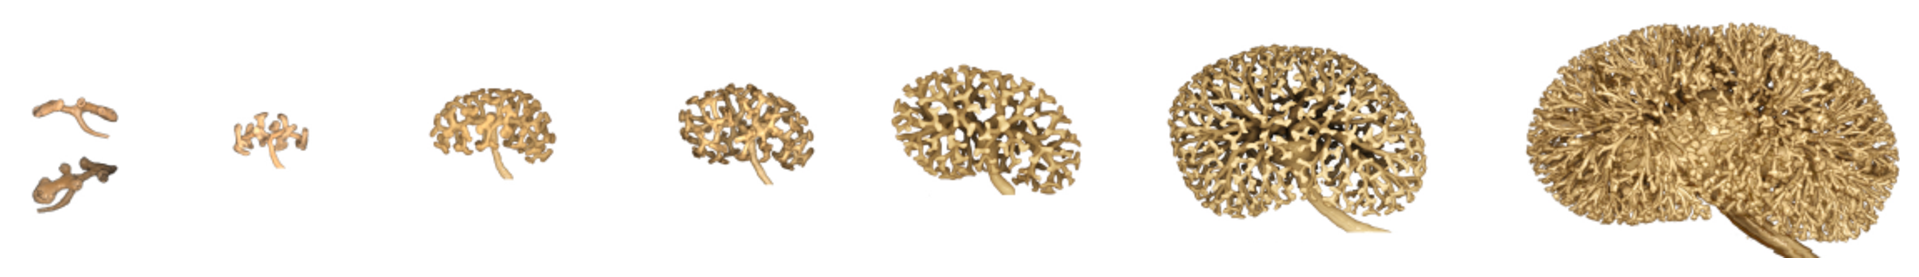
\includegraphics{real-branching.eps}}
\caption{This figure shows how the initial branching of the uretic bud (shown from two angles) on the left at E12, can, via repeated branching and elongation, lead to a highly branched structure at E16.5. This figure is taken from \cite{short2014global}.}\label{fig:real-branching}
\end{figure*} 

\section{GDNF stimulation of uretic bud growth} \label{sec:GDNF}
A range of chemical signals produced by the metanephric mesenchyme stimulate the growth of the uretic bud into the space occupied by the MM, and these have been reviewed comprehensively~\cite{costantini2006gdnf}, ~\cite{dressler2006cellular}. One of the most important of these factors is glial derived neurotrophic factor (GDNF), with GDNF$^{-/-}$ mutant mice not typically producing uretic buds. Furthermore, this factor is the morphogen associated with driving branching of the uretic bud.

GDNF is produced by the MM, and acts paracrinally on the epithelium; likely binding with two membrane surface Ret receptors (along with a co-receptor GFR$\alpha 1$) ~\cite{MenshykauDIber}. Ret$^{-/-}$ mice, like GDNF$^{-/-}$ mutants, (as well as GFR$\alpha 1$$^{-/-}$), fail to develop uretic buds ~\cite{CostantiniFKopan2010},\cite{majumdar2003wnt11},\cite{treanor1996characterization}, suggesting that these factors induce the initial growth of the epithelium into the MM.

The chemo-attractive characteristics of GDNF ~\cite{tang2002ureteric},\cite{tang1998ret}, have led to suggestions that initial growth of uretic bud, as well as subsequent branching, is due, in part, to growth and movement of epithelium towards local GDNF sources \cite{sariola2003novel}. Furthermore, explanted epithelial cells have also been shown to grow additional uretic buds in the presence of beads soaked in GDNF \cite{pepicelli1997gdnf}. 

Ret has been shown to upregulate its own expression within the epithelium, as well as production of Wnt11\cite{pepicelli1997gdnf}; Wnt11 then regulates production of GDNF by the metanephric mesenchymal cells ~\cite{majumdar2003wnt11}. Thus production of GDNF exists in a feed-forward network, with reciprocal interactions between the epithelium and the mesenchymal cells (see figure \ref{fig:pathways}). GDNF expression is however tempered by a negative feedback loop involving \textit{Sprouty1} ~\cite{basson2005sprouty1}. FGF proteins have also been implicated in stimulating the emergence of the initial uretic bud, as well as branching, although it is likely that this process is less important than the GDNF mechanism, since FGFR2${^{-/-}}$ mutants still undergo branching, albeit at a reduced level ~\cite{sims2009three}. However, in \textit{Sprouty1}${^{-/-}}$ mice, hyper-expression of FGF signalling proteins can generate phenotypically normal kidneys in GDNF$^{-/-}$ and Ret$^{-/-}$ mutants; which otherwise would have failed to develop kidneys. Since both Ret/GDNF and FGF10/FGFR have the same downstream targets ETV4/ETV5, it is likely that they may fulfil similar functions. Such redundancy could potentially have benefits evolutionarily.

\begin{figure*}[t] 
\centering
\scalebox{0.35} 
{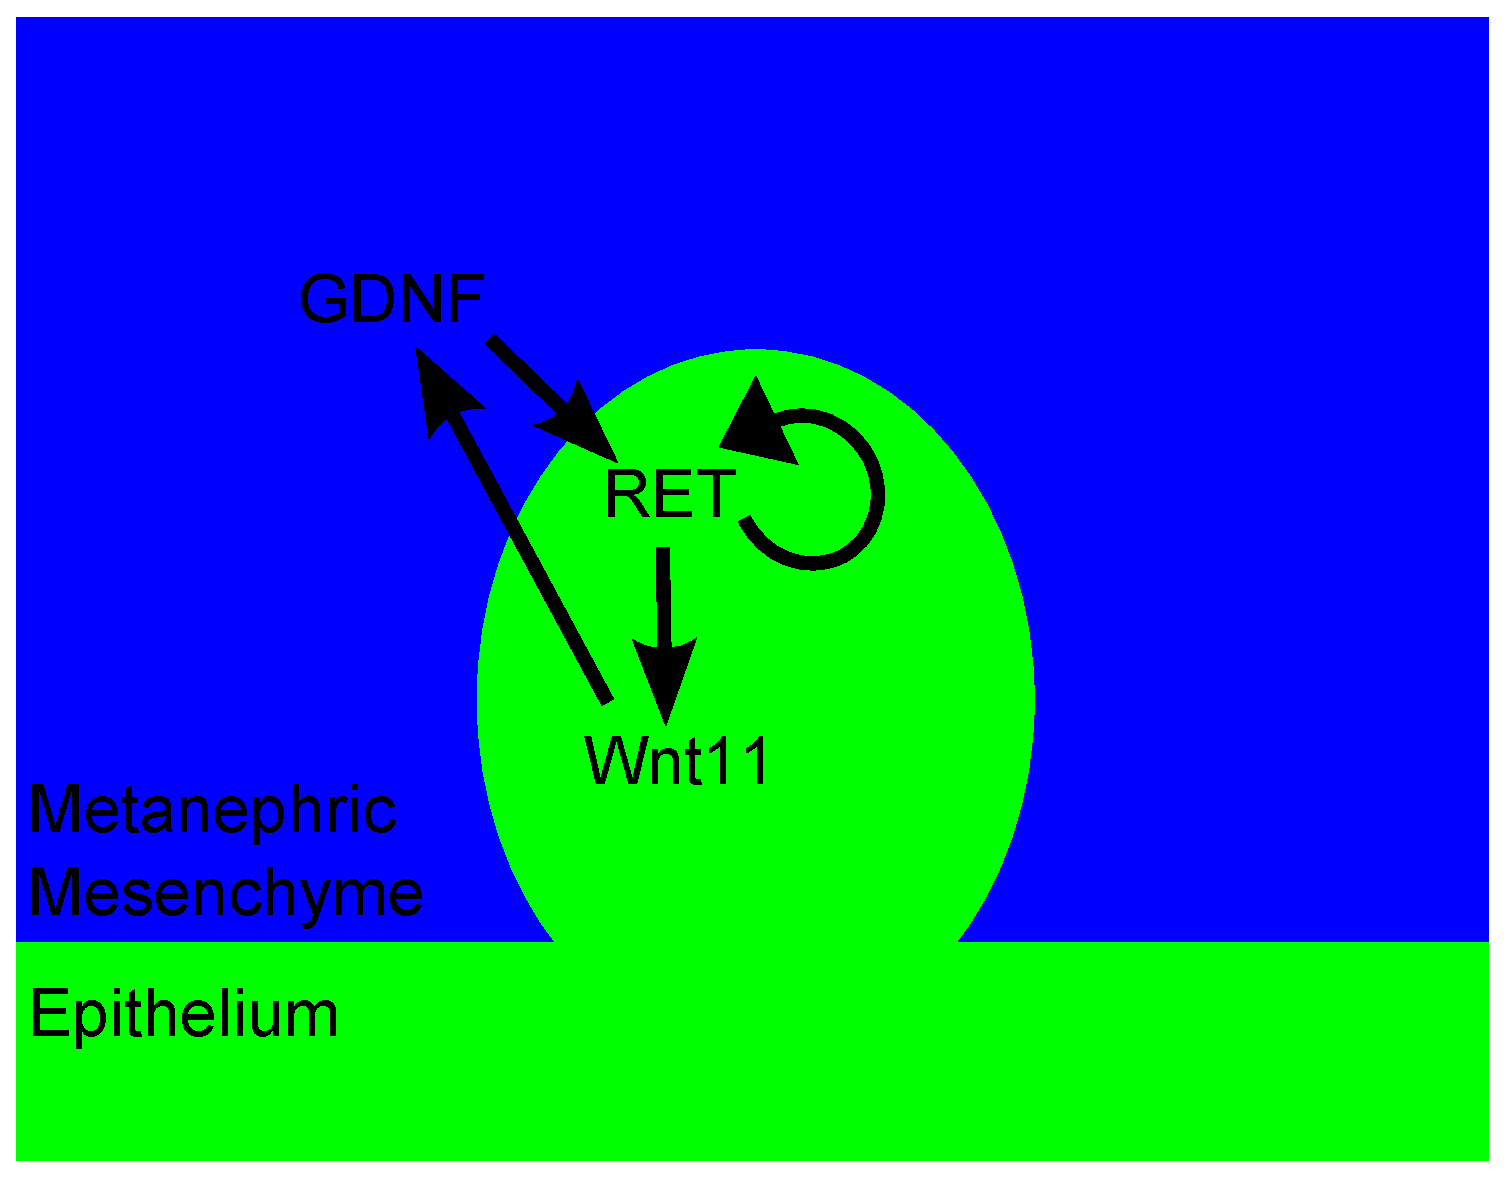
\includegraphics{pathways.eps}}
\caption{Shows the dominant reaction pathway for the regulation of GDNF in the developing kidney.}\label{fig:pathways}
\end{figure*} 

\section{Branching hypotheses}\label{sec:branchinghyp}
When the UB has invaded the MM, it undergoes approximately ten rounds of branching ~\cite{srinivas1999expression}. Thereafter the collecting duct lengthens notably, with one or two final rounds of branching before parturition ~\cite{cebrian2004morphometric}.

Branching of an emergent UB tip occurs in the absence of mesenchyme in explanted epithelial cells ~\cite{qiao1999branching}, provided the culture medium contains GDNF, as well as medium derived from cells from the early metanephric mesenchyme. Also, the branching morphology obtained with \textit{in vitro} explants is not the same as \textit{in vivo} patterning, suggesting that the mesenchyme-epithelium interaction at least plays a supporting role in kidney morphogenesis. Furthermore, experiments have been conducted whereby an explanted kidney epithelium is induced to branch like a lung, in the presence of lung mesenchyme \cite{lin2001induced}. However, the mesenchyme-independent branching result is suggestive that an important mechanism for branching is cell-contact-independent.

\begin{figure*}[t] 
\centering
\scalebox{0.2} 
{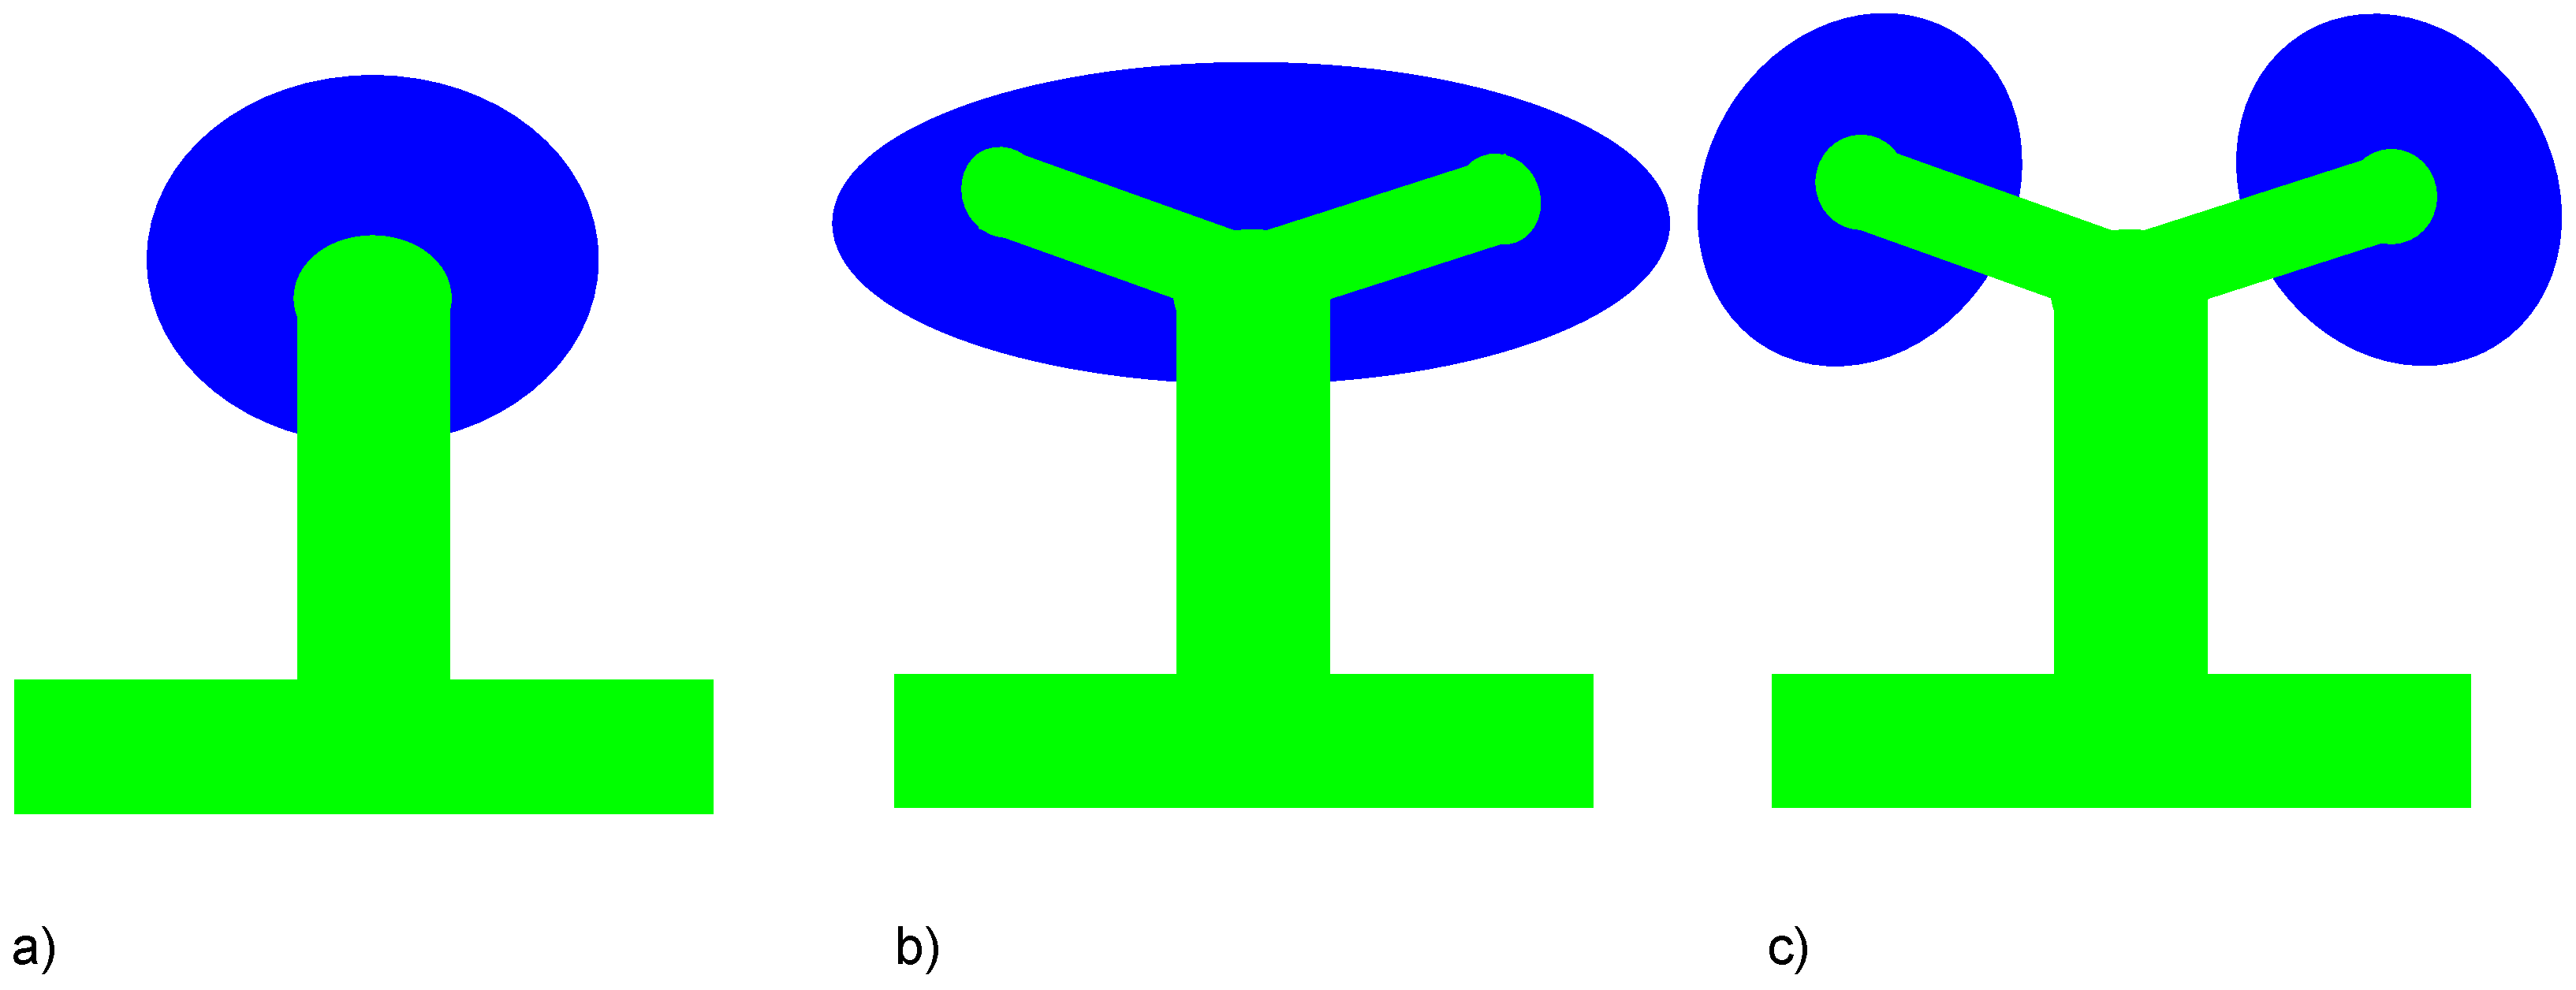
\includegraphics{UB_branch.eps}}
\caption{\textit{in vivo} branching, starting with an emergent UB in (a), initial branching occurring in (b), with discrete lobes of mesenchyme forming around epithelium tips in (c).}\label{fig:branch}
\end{figure*} 

The branches which form have (relatively) discrete masses of Six2$^+$ mesenchyme around their tips, with 'trunk' regions lacking the same mesenchyme coverage \cite{short2014global}. It is not clear whether this is indicative of all mesenchymal cells, or simply those that are Six2$^+$. However, as a first approximation it may be important for a model of branching to generate these discrete lobes of mesenchyme around tip regions of epithelium, as shown in figure \ref{fig:branch}. 

The mechanisms which lead to the branching of epithelium both \textit{in vivo} and \textit{in vitro} are not well understood. The simplest hypothesis is that branching occurs as a result of local maxima and minima in GDNF, with epithelial cells 'attracted' towards the former \cite{sariola2003novel}. Continuum models which aim to recreate the positive feedback cycle shown in figure \ref{fig:pathways}, and allow growth of epithelium at a rate proportional to GDNF concentration, have been shown to recapitulate some aspects of the branching seen \textit{in vivo} ~\cite{MenshykauDIber}. However, there are a number of issues with this approach. Firstly, if this system were allowed to continue to run, it would not necessarily reach a steady state where branching ceases, as is witnessed \textit{in vivo}. Secondly, although Ret is assumed to have a much lower diffusion rate than GDNF, since the former is a membrane protein, it is not clear whether free diffusion of Ret is a good assumption here. 

In reviewing potential mechanisms for branching Costantini and Kopan \cite{CostantiniFKopan2010} cast doubt on whether local proliferation of epithelial cells at the tips is an important mechanism since, "Mitotic events are diffusely distributed around the ampulla \cite{michael2004pattern}". They go on to suggest three further mechanisms that could be the key to generating branching:

\begin{itemize}
\item Cell movements within the epithelium
\item Orientated cell division
\item Changes of cell shape
\end{itemize}

\begin{figure*}[t] 
\centering
\scalebox{0.2} 
{\includegraphics{UB_branch_ret.eps}}
\caption{\textit{in vivo} branching with Ret-high (in red) and Ret-low (in orange) shown.}\label{fig:branch_ret}
\end{figure*} 

The first of these three mechanisms is supported by the evidence that before a UB emerges, the epithelial cells sort themselves according to their level of Ret expression \cite{Chi2009}. Before the bud emerges, the Ret-high cells gather around the position of the future bud, then go on to form the tips of the UB. Ret-activity is necessary for epithelial cells to remain at the branching tips, as well as maintain branching capacity \cite{Chi2009}. Although Ret-based sorting is evidently a part of \textit{in vivo} branching, it is still unclear how this mechanism would generate the branching that is seen. However, the discrete lobes of Six2-expressing mesenchyme which form around the tips (avoiding the trunks) could perhaps be explained by a different set of interactions between the Ret-high epithelium and the mesenchyme vs the Ret-low (see figure \ref{fig:branch_ret}).

Orientated cell division could potentially cause branching, and is supported by the finding that tip cells proliferate in a different mechanism to those in the trunks ~\cite{packard2013luminal}. When the tip cells undergo mitosis, they produce a daughter cell in the lumen, which then reinserts somewhere into the epithelium not contiguous with the parent. Whereas trunk cells produce daughter cells which are adjacent to their parents \cite{packard2013luminal}.

Changes in cell shape may also cause branching \cite{Meyer2004}. Here a "purse-string" model is proposed, whereby a cell changes shape, and due to the mechanical effect of the microfilaments in epithelial cells, this can cause 'kinks' in the epithelium, resulting in branching (see figure \ref{fig:kink}).

\begin{figure*}[t] 
\centering
\scalebox{0.4} 
{\includegraphics{kink.eps}}
\caption{An illustration of how a change in a cell's shape (coloured red), can cause folds in the epithelium to form.}\label{fig:kink}
\end{figure*} 


As well as the qualitative aspects of branching that should be replicated, there are quantitative results which a successful model of kidney morphogenesis should be able to reproduce. Throughout developmental time, there are increases in both the number of epithelium tip and mesenchymal cells located in caps around the tips, although the rate of increase of the former is lower than the latter \cite{short2014global}. This results in a decrease in the ratio of the tip to cap cells throughout this time period.

Branching of the kidney appears to stop at around birth, and it is not clear whether this is due to the release of an inhibitory factor, or whether this is the result of a gradual depletion of the self-renewing fraction of cap mesenchyme cells \cite{LittleMMcMahon2012}.

In summary, there are a number of mechanisms which are proposed for branching, although currently experiments have failed to establish which (if any) of these is the primary driver of branching.

\section{Differentiation of mesenchyme into nephron progenitors}\label{sec:differentiation}
The nephrons of the kidney are formed when the mesenchymal cells surrounding tips of epithelium differentiate via a mesenchyme-to-epithelium-transition (MET) \cite{CostantiniFKopan2010}, \cite{LittleMMcMahon2012}. These epithelial cells then become renal vesicle cells, which attach themselves to the tips, and serve as progenitors for nephrons \cite{short2014global}. 

The mesenchymal cells which originally form around the tips are at a higher density than that of the surrounding MM, and are often termed the capping mesenchyme \cite{LittleMMcMahon2012}. The mesenchyme around tips is not homogeneous. Six2 expression in particular appears to depend on the location of the mesenchyme cell, and has been demonstrated to be an important factor for maintaining mesenchyme cell pluripotency \cite{LittleMMcMahon2012}. In particular, Six2 knockout experiments in mice have demonstrated that there is premature transition of mesenchyme to renal vesicle progenitors; meaning nephrogenesis is severely impaired \cite{self2006six2}.

A number of signalling pathways have been suggested for inducing the transition of mesenchyme to epithelial cells. In mice Wnt9b signalling has been demonstrated to be the primary pathway for this induction \cite{LittleMMcMahon2012}, in particular isolated MM cells can be made to form renal vesicles in the presence of Wnt9b \cite{carroll2005wnt9b}. It is likely that Wnt9b is produced in the epithelium, and acts paracrinally on the surrounding mesenchymal cells. Since Six2 is required for mesenchymal cells to maintain their pluripotency, it is possible that a mechanism exists whereby Six2 acts to block the action of Wnt9b; preventing the cell differentiation into RVs \cite{LittleMMcMahon2012}. This would also explain why RVs tend to form in the 'armpit' region of branches, where the mesenchymal cells are surrounded by epithelium, and hence are exposed to the highest concentrations of Wnt9b.

\section{Cellular automaton model formulation}\label{sec:cellularaut}
A simple 2-dimensional cellular automaton model is presented where individual cell behaviour is dictated by the identities of nearby cells and the local concentration of GDNF. Rules are chosen to dictate cell-cell interactions in order to replicate observed behaviour. The cells are also all assumed to be the same size. These rules are over-simplifications of both the biological and physical mechanisms that govern the development of the kidney \textit{in vivo} and \textit{in vitro} for explants. However, it is hoped that the insight which this simple model can provide will be useful nonetheless for constructing more biologically and physically realistic models, where cellular behaviour is governed by physical laws rather than arbitrary rules. The model introduced here is an attempt to recapitulate branching and resultant mesenchyme distributions using as few restrictive assumptions, and rules, as is possible.

\subsection{Basic model description}
The primary aim of this model is to recapitulate the development of the uretic bud \textit{in vivo} in 2D. However, it is also hoped that the model may be applicable to \textit{in vitro} explants. The details of the model are described in brief below:
\begin{itemize}
\item A 2 dimensional rectangular domain, with $0<x<L_x$ and $0<y<L_y$, is discretised into sites of equal area. Each of these sites is assumed to be single occupancy, where each point in the array either represents the presence of:
\begin{itemize}
\item Epithelial cells - which consume GDNF, which stimulates their growth and movement. There are two types of epithelium: Ret-low and Ret-high, with the latter being more strongly stimulated by GDNF. 
\item Metanephric mesenchymal cells (MM) - which produce GDNF, and are stimulated to move and proliferate the closer they are to Ret-high epithelium. MM can also be moved out of the way by encroaching epithelium.
\item Extracellular matrix (ECM) - equivalent to 'empty space'; which allow for free diffusion of GDNF.
\end{itemize}
\item Epithelial cells comprising either:
\begin{itemize}
\item A \textit{flat} membrane at the base of the simulation domain (aimed at recapitulating the \textit{in vivo} conditions from which the UB initially forms \textit{in utero}.)
\item A mass of epithelial cells with in general, curved boundaries, suspended towards the centre of the simulation domain (representative of the \textit{in vitro} explant experiment initial conditions.)
\end{itemize}
\item A diffuse collection of mesenchymal cells initially separate from the epithelium for the \textit{in vitro} case, and a concentrated rectangular mass nearby the Wolffian duct for the \textit{in vivo} one.
\end{itemize}

In the model, the mesenchyme produce GDNF, which then diffuses across the domain and is consumed by epithelium; stimulating the movement and proliferation of epithelial cells. Ret-high cells are more strongly stimulated by GDNF than Ret-low. This results in an aggregation of Ret-high cells near to the mesenchyme. Furthermore, the mesenchyme are themselves stimulated to move and proliferate if they are close to Ret-high epithelium.

\subsection{GDNF field}
Cells in the MM produce GDNF, and it diffuses freely across the extracellular matrix (ECM) layer, and through the epithelium (being consumed by the latter). Since the time scale for GDNF diffusion is much less than the time scale for cell division, we use a quasi-steady 2D RDE to model the distribution of GDNF, $G(\mathbf{x},t)$, neglecting time derivatives so that we have:

\begin{equation}\label{eq:RDE}
\frac{\partial G}{\partial t} \approx 0 = D_G \nabla^2 G - \Phi_G
\end{equation}

In (\ref{eq:RDE}) $D_G$ denotes the diffusion coefficient for GDNF, and $\Phi_G$ is the net local rate of GDNF production. Specifically the rate of GDNF consumption is assumed to have the following form:

\begin{equation} \label{eq:production}
\Phi_G =\begin{cases}
K_G G, & \text{for epithelium}.\\
-\rho_G, & \text{for mesenchyme}.\\
0, & \text{for the extracellular matrix}.
\end{cases}
\end{equation}

For simplicity we assume that the rate of GDNF consumption is linearly-dependent on the concentration of substrate. In future work, it may be better to assume a Hill-type reaction rate \cite{MenshykauDIber}. (Although it is unclear what range of concentrations of GDNF are likely to saturate the Ret receptors, and whether these are likely to be encountered \textit{in vivo} or \textit{in vitro}.) For simplicity we assume that mesenchymal cells produce GDNF at a constant rate $\rho_G$, although we realise that in practice that this rate is up-regulated by Wnt11 (see figure \ref{fig:pathways}). However, \textit{in vivo} this positive feedback mechanism is likely tempered by the \textit{Sprouty1} pathway (which itself is not fully-understood), and in \textit{in vitro} experiments without mesenchyme, branching occurs regardless. As such, the model presented here omits this feedback mechanism for simplicity.

We impose no flux boundary conditions on $x=0$, $x=L_x$ and periodic boundary conditions at $y=0$ and $y=L_y$. The simulation domain is chosen to be sufficiently large however, such that edge effects do not influence the resultant behaviour.

(\ref{eq:RDE}) is non-dimensionalised using the following transformations:
\begin{equation}\label{eq:difftrans1}
\eta = \frac{x}{\Delta}, g = \frac{G}{G_x}
\end{equation}


In (\ref{eq:difftrans1}) $\Delta$ refers to the typical cell dimensions (approximated as 5 $\mu m$),and $G_x$ is the concentration of GDNF typically found \textit{in vivo}. These transformations result in the following non-dimensional form of the steady-state reaction-diffusion equation:

\begin{equation}\label{eq:diff-dimensionless}
\nabla_\eta^2 g = \frac{\phi_g}{d_g}
\end{equation}

In (\ref{eq:diff-dimensionless}), $d_g = \frac{D_G}{K_G \Delta^2}$, $\phi_g = \frac{\Phi_G}{K_G G_x}$, and $\nabla_\eta^2$ is the laplacian in the non-dimensional $\eta$ spatial coordinates.

\subsection{Cell based rules}
In this section a brief description of the cell based rules are provided, with a more complete description provided in section \ref{sec:rules}, in the appendix. 

\subsubsection{Updating of cells at each time step}\label{sec:updateall}
At each time step of the simulation the cell identities (Ret-high and Ret-low epithelium, as well as mesenchyme) are collected, and randomly sorted into a list. All the cells are then visited once, and updated (see figure \ref{fig:algorithm}). When each epithelial cell is visited, it is first established whether there are available adjacent sites into which the cell can either move or produce a daughter cell (for proliferation). If there are no available sites, then the next cell in the list is selected. If there are available sites, then based on $P_{move}$ a move or a proliferation event is implemented. For epithelial cells, a further step is implemented, which is termed 'Ret-transformation'. This describes the process whereby a Ret-low cell can probabilistically transform into a Ret-high cell (and vice versa), based on the local GDNF concentration (see section \ref{sec:mesenchyme}). This process is absent for mesenchyme. Finally, the next cell in the list is selected. In simulations $P_{move}=0.5$ so that there was an equal probability of moving or proliferating.

\begin{figure*}[t] 
\centering
\scalebox{0.8} 
{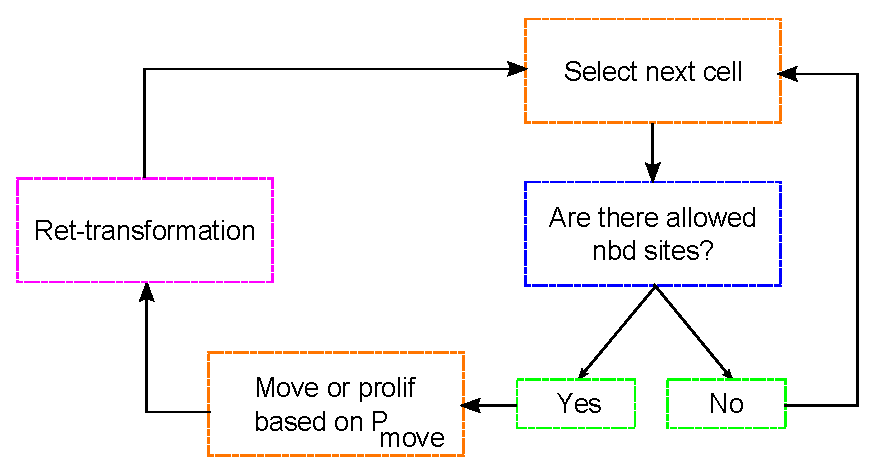
\includegraphics{algorithm.eps}}
\caption{A schematic of the algorithm used to update all cells at each time step. This loop is continued across all cells, until each one in the list has been visited. $P_{move}$ is chosen to be 0.5, so that there is equal weighting of movement and proliferation. The 'ret-transformation' step is only implemented for epithelium.}\label{fig:algorithm}
\end{figure*}

\subsubsection{Implementing a move or a proliferation event}
After it has determined that a \textit{move} or \textit{proliferation} event be considered, a set of rules dictate whether this particular event takes place, and, if so, determines into which site the cell should move or produce a daughter cell (see figure \ref{fig:algorithm_specific}). The reasoning for retaining the possibility of an event not occurring, is to allow the probability for event rates to be determined by local GDNF concentration, and in particular, to allow this to be different for moving and proliferating respectively. 

After a given action (moving or proliferating) has been selected, (see section \ref{sec:updateall}), firstly a probability of the action, $P_a$ is calculated. This is a function of the local GDNF level for epithelium (see section \ref{sec:prob}), or a function of the distance of the nearest Ret-high epithelium for mesenchymal cells (see section \ref{sec:mesenchyme}). A pseudorandom uniform number between 0 and 1, is then compared with $P_a$ to determine whether the action is implemented for that epithelial cell. The probability of an action occurring for a Ret-high cell is chosen to be higher, at a given local concentration of GDNF, than a corresponding Ret-low cell. This was chosen so that Ret-high cells aggregate around GDNF-rich tips, with Ret-low cells towards 'stalk' regions.

If an action is chosen to be implemented, a site must be chosen into which the active cell will move or produce a daughter. Introducing movement/proliferation which is directed towards sites of higher GDNF was found not to significantly affect the qualitative branching patterning (see sections \ref{sec:target} and \ref{sec:mesenchyme}). As such, this mechanism was neglected in generating results; with sites being chosen uniformly at random from the list of the available.

\begin{figure*}[t] 
\centering
\scalebox{0.7} 
{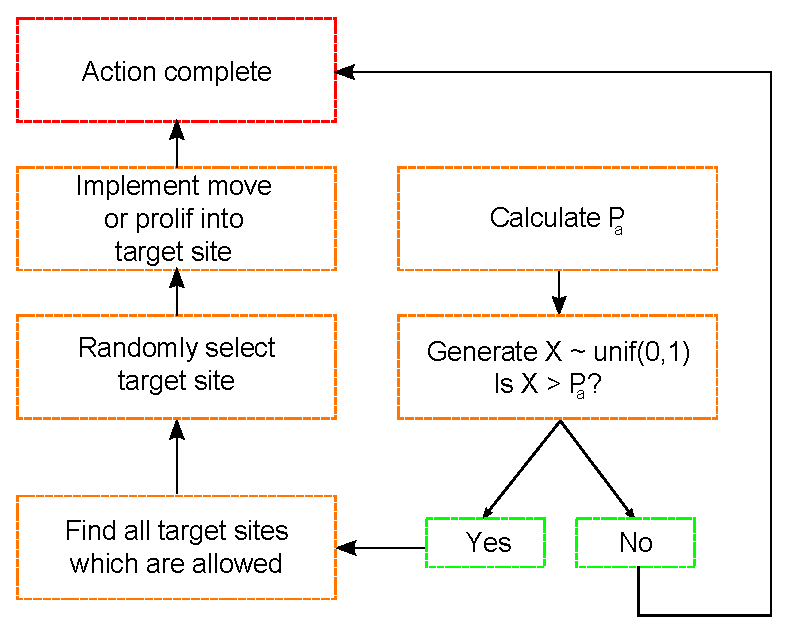
\includegraphics{algorithm_specific_nochemo.eps}}
\caption{A schematic of the algorithm used to choose whether a move or proliferation occurs, and, if so, guide its implementation.}\label{fig:algorithm_specific}
\end{figure*}

\subsection{Numerical simulation}
The GDNF concentration field is numerically solved at each time step, using a finite difference approximation, with the grid discretisation points corresponding to the cell centres. The details of this are found in section \ref{sec:GDNFfield} in the appendix. It is assumed that changes in location of cells within each time step are sufficiently small to not cause significant differences in the resultant GDNF field, and as such, the field is only updated at the beginning of each time step.

The cells are then visited once each time step, in a randomised order, and are updated according to the aforementioned rules. The simulations were conducted using Matlab 2014a, on a Windows XP computer.

\section{Results}\label{sec:results}
\subsection{In vivo}\label{sec:quantresults}
A typical simulation consisted of an initial rectangular layer of 4,000 epithelium cells, consisting of 10\% Ret-high and 90\% Ret-low, and a separate rectangular layer of mesenchymal cells (see figure \ref{fig:emergent}). The mesenchyme induces transformation of nearby Ret-low cells into Ret-high cells. Furthermore, Ret-high cells outcompete Ret-low cells to move closer to the mesenchyme. This results in an initial aggregation of Ret-high cells near the mesenchyme, before the emergence of the uretic bud. 

Branching was generated \textit{in silico} if restrictions were placed was placed on the non-local movements of the mesenchymal cells (in both the primary and secondary axes directions as defined in section \ref{sec:mespassive}). Physically, this represented a constraint on the maximal number of mesenchymal cells which an encroaching epithelium cell layer can move out of the way; leading to a 'bottle-neck' in the middle of the emergent uretic bud, and two terminal branches on either side (see figure \ref{fig:emergent}).

\begin{figure*}[t] 
\centering
\scalebox{0.93} 
{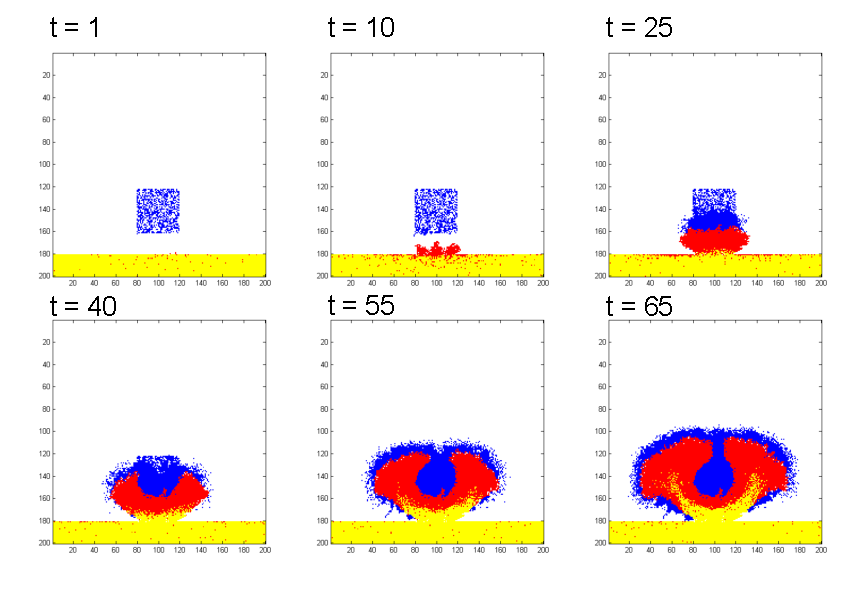
\includegraphics{emergent.eps}}
\caption{Depicts the emergence of a uretic bud across simulation time. Mesenchymal cells are coloured blue, with Ret-high epithelum in red, and Ret-low in yellow. Here mesenchyme were allowed to be moved non-locally 10 cells forward along the principal axis and 2 cells either side along the secondary axis.}\label{fig:emergent}
\end{figure*} 



\textit{In silico} experiments were conducted in which the width and depth of the mesenchyme layer were varied. As the depth or width of mesenchyme was increased, \textit{ceteris paribus}, this increased the width of the emergent uretic bud, due to higher concentrations of GDNF at the epithelium boundary. This is reminiscent of earlier \textit{in vitro} experiments, where multiple UBs have been shown to form in the presence of higher GDNF concentrations \cite{pepicelli1997gdnf}. At the opposite side of the scale, when the initial number of mesenchymal cells falls below a certain number (which depends on the sensitivity of epithelial cells to GDNF concentration), then genesis of a uretic bud may not occur, or take longer to emerge. The results of the sample simulations with differing initial numbers of mesenchyme are shown in figure \ref{fig:initial}.

\begin{figure*}[t] 
\centering
\scalebox{0.93} 
{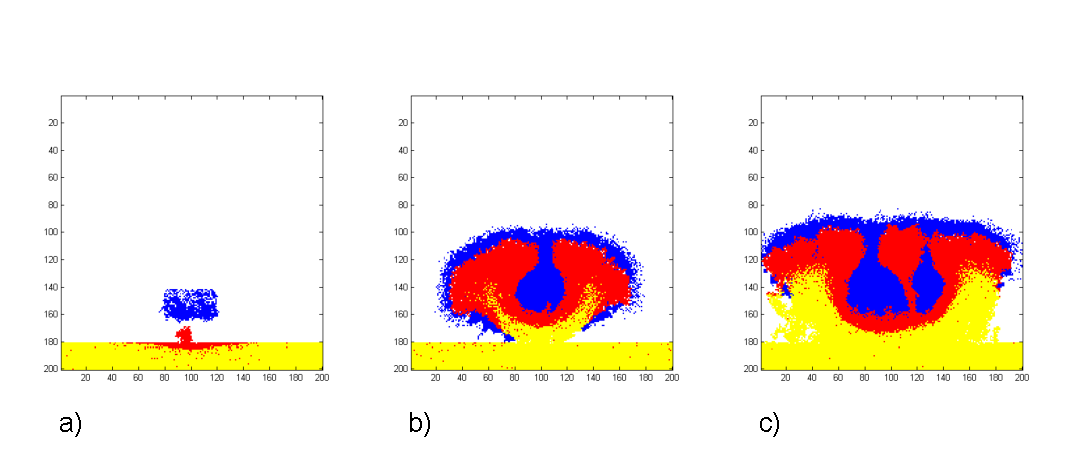
\includegraphics{initial.eps}}
\caption{Displays the effect of changes in the initial numbers of mesenchyme on the width of the emergent uretic bud after 65 simulation time steps. As the number of mesenchymal cells initially increases from a) to c), the width of the uretic bud increases. Mesenchymal cells are coloured blue, with Ret-high epithelum in red, and Ret-low in yellow.}\label{fig:initial}
\end{figure*} 

Increases in the depth and width of the mesenchyme layer were also found to hasten the time at which branching occurs. \textit{In silico} this is because beyond a certain critical distance either in the primary axis or secondary axis directions (as defined in figure \ref{fig:axes}), the mesenchyme can no longer be 'pushed' out of the way by encroaching epithelium. It is thought that the mesenchyme will most likely move in a direction aligned with the direction in which they were pushed, thus suggesting that the maximal distance along the primary axis a mesenchyme can be non-locally moved should be greater than that along the secondary axis. If this is assumed in the simulation, then initial branching of the emergent bud is more sensitive to changes in the depth of the mesenchyme than the width. In particular greater depths cause branching to occur earlier in terms of simulation time, and can moderate the branching angle. Intuitively, greater mesenchyme depths exert a larger pressure on the encroaching epithelium, and hence favour lateral growth of the epithelium. The angle of branching is reduced, the greater the depth of the mesenchyme, since the individual branches continue to be attracted up the length of the mesenchyme layer. Examples of this angular difference in branching are shown in figure \ref{fig:depth}.

\begin{figure*}[t] 
\centering
\scalebox{1.0} 
{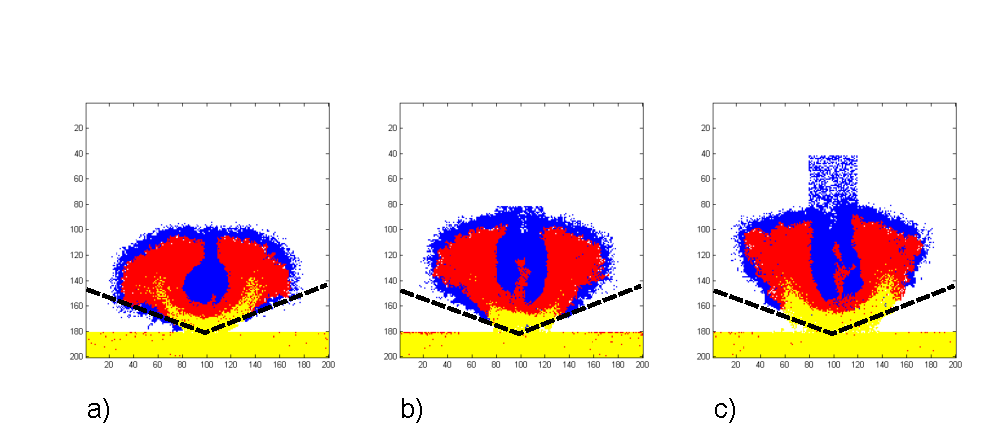
\includegraphics{depth.eps}}
\caption{Displays the effect of changes in the mesenchyme depth on the subsequent branching angle. As the depth increases from a) to c), the angle which the subsequent branches form with one another decreases. The angle which the outermost epithelium cells make with the centre of the UB for case a) is superimposed on b) and c). Mesenchymal cells are coloured blue, with Ret-high epithelum in red, and Ret-low in yellow.}\label{fig:depth}
\end{figure*} 

\begin{figure*}[t] 
\centering
\scalebox{1.0} 
{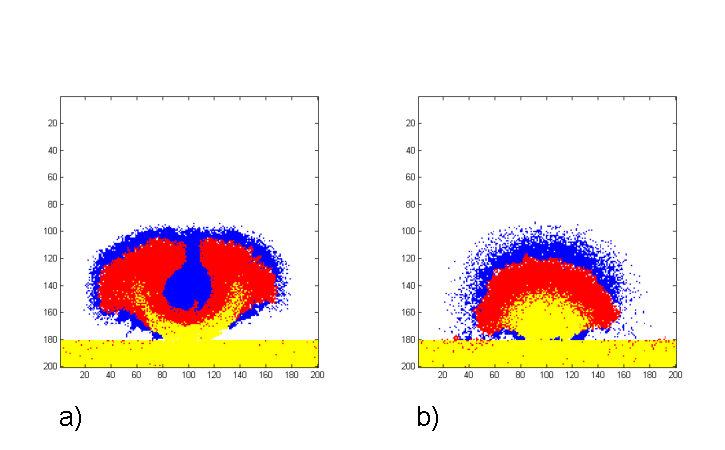
\includegraphics{shell.eps}}
\caption{Compares the morphologies which result in a) where the mesenchyme exerts a 'pressure' on the encroaching epithelium, with b) where there is no such 'force'. Mesenchymal cells are coloured blue, with Ret-high epithelum in red, and Ret-low in yellow.}\label{fig:shell}
\end{figure*} 

It is unlikely that this mechanism is the principal cause of branching \textit{in vivo}, since the mesenchyme are relatively diffuse. Thus mesenchymal cells are unlikely to exert a sufficiently strong enough force on the wave of encroaching epithelium to halt the centre of the wavefront; allowing the growth laterally. Furthermore, \textit{in vitro} studies with explanted epithelial cells without mesenchyme have demonstrated that branching can continue to produce self-similar tips if GDNF is present \cite{qiao1999branching}. These two reasons cast serious doubt on this as a likely primary cause of branching. An example simulation where the simulation pressure has been removed is shown in figure \ref{fig:shell}, where it is evident that without this feature, branching fails to occur. The pressure is removed by allowing the mesenchymal cells to be moved large distances non-locally along both the principal and secondary axes. However, it may be the case that the pressure provided by the surrounding mesenchyme cap moderates the morphology of the developing UB, since the \textit{in vivo} and \textit{in vitro} branches are not the same.

We also investigated the quantitative relationship between the final number of epithelial cells forming part of the uretic bud and the initial characteristics of the mesenchyme block. This was suggested \footnote{By Melissa Little and Helen Byrne.} as a potential basis around which future experiments can be constructed in order to test the foundations of the cellular automaton model presented here. Figure \ref{fig:nums} shows the decreasing returns to numbers of initial mesenchyme cells in terms of the number of epithelium cells forming part of the uretic bud after 35 time steps \footnote{The parameters for used for the simulation are stated within section \ref{sec:parameters}.}. Due to the nature of this ever-decreasing relationship, there is an optimal ratio of mesenchyme cells to epithelium which results in the highest inverse ratio at the end of simulation (see figure \ref{fig:nums_increment}). Furthermore over the range of parameters chosen, increases in the width and depth of the initial mesenchyme layer do not appear to have a different effect of the final numbers of epithelium which form part of the uretic bud (see figure \ref{fig:heat}). This difference was tested statistically via a linear regression of the form\footnote{The squares of the variables were included in order to control for diminishing returns of both variables to final epithelium number observed in figure \ref{fig:nums}.}:

\begin{equation}\label{eq:testreg}
E = \alpha + \beta_1 W + \beta_2 (W + D) + \beta_3 W^2 + \beta_4 D^2
\end{equation}

In (\ref{eq:testreg}), $E$ refers to the number of epithelium cells in the UB at the end of the simulation period, $W$ and $D$ are the initial width and depth of the mesenchyme 'rectangle' in the simulation domain. The coefficient $\beta_1$ was found to be statistically-insignificant at the 5\% test size; suggesting that there was no difference between the effect of changes to the width and depth of the mesenchyme layer at simulation start.



\begin{figure*}[t] 
\centering
\scalebox{1.0} 
{\includegraphics{cell_numbers.eps}}
\caption{Shows the relationship between the initial number of mesenchymal cells to the final number of epithelium cells which form part of the uretic bud after 35 time steps. The red regression line was estimated using least squares regression with a quadratic polynomial in terms of the initial mesenchyme, with the average of 8 simulations at each parameter value resulting in the recorded epithelium. The green error lines were the result of fitting the same type of regression using the epithelium average plus/minus one standard deviation at each parameter value.}\label{fig:nums}
\end{figure*} 

\begin{figure*}[t] 
\centering
\scalebox{1.0} 
{\includegraphics{cell_numbers_increment.eps}}
\caption{Shows the relationship between the initial number of mesenchymal cells to the number of epithelium cells at the beginning of the simulation to the inverse relationship after 35 time steps. The red fitted line was estimated using a least squares spline method. The green error lines were the result of fitting the same type of regression using the epithelium average plus/minus one standard deviation at each parameter value.}\label{fig:nums_increment}
\end{figure*}

\begin{figure*}[t] 
\centering
\scalebox{0.8} 
{\includegraphics{heat_map.eps}}
\caption{A heat map showing the relationship between width and depth of the initial rectangular mesenchyme block, to the final number of epithelium cells which form part of the uretic bud \textit{in silico} after 35 time steps. The darker the colour, the higher the final number of epithelium cells.}\label{fig:heat}
\end{figure*}  

\subsection{In vitro}
Symmetry is already broken \textit{in silico} for the initial transplanted epithelium mass. As a result branch formation could be initiated due to local minima in GDNF forming in clefts, and maxima forming at the outermost edges of the epithelium layer. The GDNF-rich tips of the epithelium grew fastest. By contrast those cells in GDNF-low pockets failed to grow since the surrounding epithelial cells had consumed a relatively high proportion of the GDNF. These tips hence became tentacles, extending outwards from the initial mass of epithelial cells. Example \textit{in silico} visualisations of this process are shown in figure \ref{fig:invitro_emerge}.

\begin{figure*}[t] 
\centering
\scalebox{1.0} 
{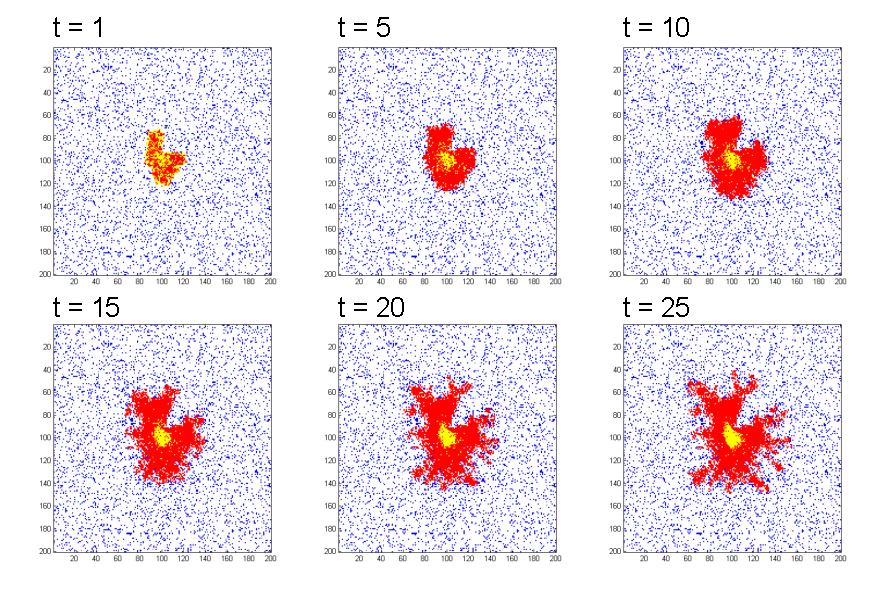
\includegraphics{invitro_emerge.eps}}
\caption{\textit{in vitro} framework investigated \textit{in silico} using the cellular automaton model. Mesenchymal cells are coloured blue, with Ret-high epithelum in red, and Ret-low in yellow.}\label{fig:invitro_emerge}
\end{figure*} 

\textit{In silico} simulations where two explanted kidney uretic buds are placed near to one another in a tissue culture are shown in figure \ref{fig:duo}. The resultant patterning shows that there is branching on the sides of the explants which face away from one another. This morphology results \textit{in silico} because local minima of GDNF on those inwards facing sides surpress growth there. It would be interesting to compare these results with those obtained from \textit{in vitro} experiments, in order to ascertain whether the local GDNF concentration causes branching.

\begin{figure*}[t] 
\centering
\scalebox{1.0} 
{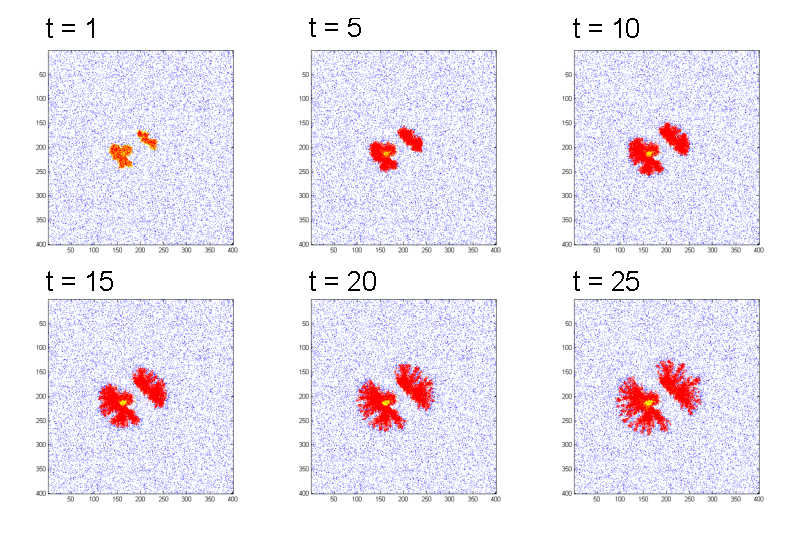
\includegraphics{duo.eps}}
\caption{A two explant \textit{in silico} experiment. Branching is seen on the outwards facing sides of the epithelium explants. Mesenchymal cells are coloured blue, with Ret-high epithelum in red, and Ret-low in yellow.}\label{fig:duo}
\end{figure*} 


Whilst branching was generated in the \textit{in vitro} simulations, the continued rounds of branching which characterise \textit{in vitro} experiments were not observed. As such, the mechanism proposed here of an asymmetric mass of epithelium generating local maxima and minima in GDNF could not replicate reality. Much like the \textit{in vivo} case, it will be necessary to investigate other causes of branching. In particular, following Costantini and Koplan \cite{CostantiniFKopan2010}, anisotrophic cell growth may hold the key to generating the  morphological patterns witnessed. This is further supported by work which suggests that there are differences between the proliferative habits of tip and trunk cells \cite{packard2013luminal}.

\begin{figure*}[t] 
\centering
\scalebox{0.9} 
{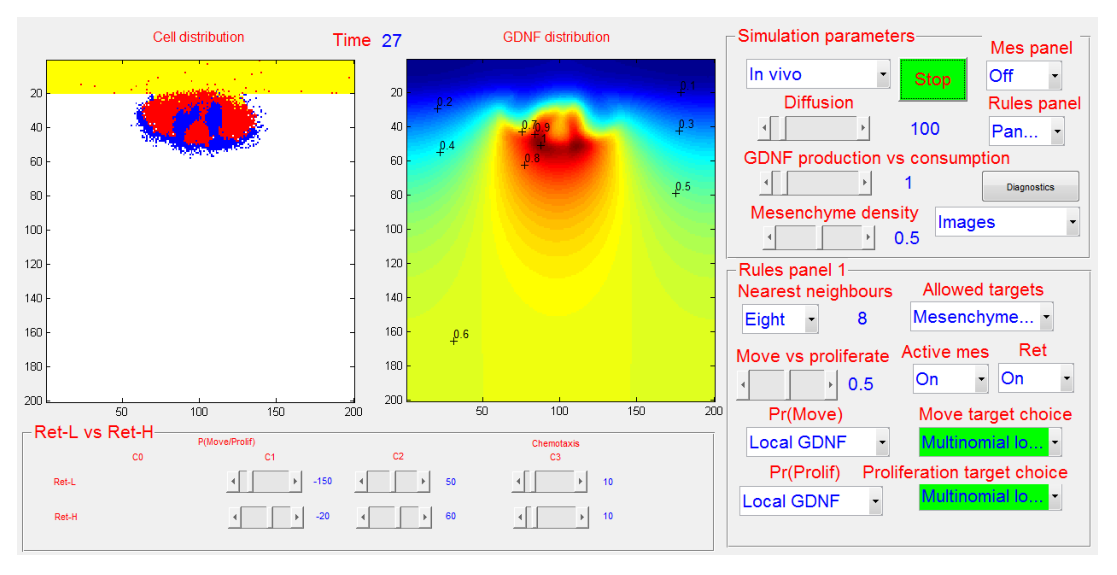
\includegraphics{gui_screenshot.eps}}
\caption{A screenshot of the software produced to allow experimental collaborators to investigate the model in terms of parameters and rules chosen.}\label{fig:gui}
\end{figure*} 


\subsection{Software}
As part of the process of producing the aforementioned model, a GUI was created which allows a user to select between the various rules, and parameter values used to dictate the movement and proliferation of cells in the system (see figure \ref{fig:gui}). Furthermore, the GUI allows a user to select between \textit{in vitro} and \textit{in vivo} experimental conditions. This is currently with experimental collaborators. It is hoped that this may stimulate further experimental work which can be used for testing of the model's assumptions and predictions.

\section{Conclusion and future work}
This paper presented a cellular automaton model which generated branching of uretic buds in both \textit{in vivo} and \textit{in vitro} conditions. However, the branching patterns that have been shown to result from simple GDNF-stimulated growth are not fully consistent with what has been observed \textit{in vivo} and \textit{in vitro}. In particular the lack of continued rounds of branching in \textit{in silico} simulations provide insight that an important mechanism has been neglected. Costantini and Koplan \cite{CostantiniFKopan2010} maintain that they believe that there are three potential mechanisms for generating the branching patterns seen in experiments: cell movements within the epithelium, orientated cell division, and changes of cell shape. We agree that all three of these mechanisms likely play a role in branching, although anisotrophic growth between the tip and cap cells may be the most important. In the model formulation presented here, lumen formation of the collecting duct has been neglected. This simplification may be important, since it may provide an axis around which epithelial cells are exposed to a range of pressures. It is possible that the differential pressures exerted on the tip and trunk cells by the lumen may explain phenotypic differences in their proliferation status, and may stimulate anisotrophic growth. Without including a lumen, it is difficult to predict how it would be possible to orientate cell division differently between the tip and trunk. Whilst it may be possible to explicitly include a lumen in a cellular automaton model, this may not be the most appropriate modelling framework to do so, and other cell-based models may be better suited. In particular, an off lattice, overlapping spheres model may be a more appropriate framework for further work.

The software produced allows experimental collaborators to easily manipulate the model's rules and parameters. It is hoped that this may result in future experiments used to test the validity of the model's assumptions.

\appendix
\section{Finite difference approximation for RDE of the GDNF field}\label{sec:GDNFfield}
(\ref{eq:RDE}) is discretised across the simulation domain. The non-dimensional GDNF concentration is determined by:

\begin{equation}\label{eq:discrete}
g_{ij} = g(i\Delta_x, j\Delta_y)
\end{equation}

In (\ref{eq:discrete}), $g(i\Delta_x, j\Delta_y)$ represents the GDNF concentration at the point in the domain specified by the coordinates $(i\Delta_x, j\Delta_y)$. Here $\Delta$ represents a cell width, and is is assumed that $\Delta_x = \Delta_y$.

The periodic boundary conditions at either side of the domain are represented by imposing the following restrictions on the GDNF field:

\begin{align*}
g_{0,j}& = g_{1,j}\\
g_{M,j}& = g_{M+1,j}\\
\end{align*}

Where this holds $\forall j = 1,...,N$. $M$ here is the depth of the simulation domain in terms of cell dimensions. Similarly, for the periodic boundary conditions:

\begin{align*}
g_{i,0}& = g_{i,N}\\
g_{i,N+1}& = g_{i,1}\\
\end{align*}

where this holds $\forall i = 1,...,M$. $N$ here is the width of the simulation domain in terms of cell dimensions.

The finite-difference approximation for solving the steady-state reaction-diffusion equation is hence of the form:

\begin{equation}\label{eq:finitediff}
g_{i+1,j} + g_{i-1,j} + g_{i,j+1} + g_{i,j-1} - (4 + \epsilon_{i,j})g_{i,j} = -\psi_{i,j}
\end{equation}

Where in (\ref{eq:finitediff}):
\begin{equation}
\epsilon_{i,j} =\begin{cases}
\frac{1}{d_g}, & \text{for epithelium}.\\
0, & \text{for mesenchyme}.\\
0, & \text{for the extracellular matrix}.
\end{cases}
\end{equation}

Also, in (\ref{eq:finitediff}):
\begin{equation} \label{eq:psi}
\psi_{i,j} =\begin{cases}
0, & \text{for epithelium}.\\
\frac{\gamma}{d_g}, & \text{for mesenchyme}.\\
0, & \text{for the extracellular matrix}.
\end{cases}
\end{equation}

In (\ref{eq:psi}), $\gamma = \frac{\rho_G}{K_G G_x}$ captures the relative rate of GDNF production by the mesenchyme compared to the rate of GDNF consumption by epithelium under normal cellular conditions. Furthermore, $D_G$ and $d_g$ represent the dimensional and non-dimensional diffusion rate for GDNF respectively. It is assumed that $\gamma = 1$ in the simulations, in the absence of information regarding the relative weight of these two mechanisms. The diffusion rate constant, $D_G$, is assumed to be 10 $\mu m^2 s^{-1}$ \cite{MenshykauDIber}. If we assume that the diffusive time scale is similar to that of GDNF consumption we find that:

\begin{equation}\label{eq:diffusiontime}
k_G \sim \frac{D_G}{L_x \times L_y} 
\end{equation}

The diffusive time scale implied by this reasoning made it significantly more difficult to generate branching in the \textit{in vitro} simulations. This was because diffusion rate acted to smooth differences in GDNF concentration across the domain, making local minima and maxima less pronounced. In practice, GDNF may not diffuse freely through the simulation domain since the domain is not empty space. We used this to justify using a lower dimensionless diffusion rate of GDNF.

In the simulation, it is assumed that the GDNF field does not vary significantly within a particular time step. As such (in order to reduce computational load), the GDNF field is only updated at the end of each time step, not after each cell movement or proliferation.

\section{Cell based rules}\label{sec:rules}
\subsection{Rules for epithelial cells}
In this section the rules governing the behaviours of the epithelial cells are described. In the algorithm, all cell locations (both mesenchyme and epithelium) are sorted into a list with a randomised order. At each time step the next cell in the list is visited, with epithelial cell behaviour governed by the following pseudo-algorithm:

\begin{itemize}
\item \textit{Available cells} - Are neighbouring sites available for movement or proliferation? If unoccupied, proceed to the next step. If no, move on to next cell. 
\item \textit{Move or proliferate} - Draw a random number $X\sim unif(0,1)$. If $P_{move}>X$ then proceed to \textit{move}. If not, proceed to \textit{proliferate}.
\item \textit{Move} 
\begin{enumerate}
\item \textit{Calculate the probability, $P_a$, that a move takes place} - Based on a function of the local GDNF concentration (see section \ref{sec:prob}).
\item \textit{Does a move take place?} - Draw a random number $X\sim unif(0,1)$. If $P_{a}>X$ then proceed to next step. Otherwise, consider next epithelium cell.
\item \textit{Calculate probability of moving to each of the available sites}.  The method used to do this is described in section \ref{sec:target}.
\item \textit{Choose amongst the available cells in accordance to their probability and move the cell in question}. (See section \ref{sec:target}.)
\end{enumerate} 
\item \textit{Proliferate}
\begin{itemize}
\item A daughter cell is chosen to move into the target cell, with the existing cell remaining static in contrast to the \textit{Move} behaviour.
\end{itemize}
\item Consider next cell, returning to first step.
\end{itemize}

A potential cause of branching behaviour highlighted by Costantini and Koplan \cite{CostantiniFKopan2010}, is differential cell movements within the epithelium. In section \ref{sec:branchinghyp}, one potential source of epithelium heterogeneity, that would cause different movement behaviours across cells, was expression of Ret. Furthermore, it was indicated that Ret-activity, specifically competition, occurs \textit{in vivo}, which results in Ret-high cells forming the initial bud, and then remaining in the tip cells \cite{Chi2009}. As such, two types of epithelium cell were created: Ret-high, and Ret-low. The former being more likely to divide and move in the presence of GDNF (see section (\ref{eq:probit})).

As well as allowing Ret-high cells to move, and proliferate into neighbouring available cells at rates which are higher than the Ret-low, in order to reproduce the initial aggregation of Ret-high cells which forms the uretic bud it was necessary to create a new type of behaviour. 'Competition' between a Ret-high and Ret-low cell, results in them swapping their positions. Successful competition can only occur only if the adjacent Ret-low cell is at a higher local GDNF concentration than the Ret-high one. The probability of swapping cell positions on the lattice is determined by a probit function of the same form as (\ref{eq:probit}), with the move more likely to occur if the target cell has a higher concentration of GDNF. In the case of where two or more Ret-low cells are adjacent to a Ret-high cell, the cell with the highest GDNF concentration is chosen to be its 'partner' in competition with probability 1.

Epithelial cell fates are not in practice determined at their genesis \cite{CostantiniFKopan2010}. Lateral branching \cite{watanabe2004real}, and MM-induced branching \cite{sweeney2008developmental}, can both occur with new tips forming from the trunk region of epithelial cells. As such, cells should be able to transform from one level of Ret expression into another. In order to allow reversible transitions, the probabilities of a transition occurring (each time a cell is updated in the simulation), are of the probit form:

\begin{equation}\label{eq:transition}
P(transition) = \Phi (c_1 + c_2 g)
\end{equation}

Where in (\ref{eq:transition}) for the two cell types: $c_2>0$ for Ret-low to Ret-high transitions; and $c_2<0$ for Ret-high to Ret-low transitions. The differential transition probabilities for both cell types at a non-zero GDNF concentration allows for the creation of Ret-high cells in newly formed tips, and the transition of cells in stalk regions to Ret-low. When an epithelium cell divides, it is chosen to be of the same type as its parent.

Finally, in order to form discrete lobes of mesenchyme around the tips (where the Ret-high cells are located), it is necessary for the mesenchyme to be attracted differentially to Ret-high and Ret-low cells respectively. Details of the rules governing this behaviour are covered in section \ref{sec:mesenchyme}.

\subsubsection{Available neighbours for epithelial cells}\label{sec:available}
An epithelium cell's neighbours were chosen to be the grid points specified by a Moore neighbourhood of 8 sites. Simulations were also run with Von-Neumann 4-cell neighbourhoods, but results were found to be almost identical.

\begin{figure*}[t] 
\centering
\scalebox{0.5} 
{\includegraphics{connected.eps}}
\caption{An explanation of 'connectivity' for epithelial cells. All cells here are epithelium, the one highlighted in red is the cell which has been moved. Moves (a) and (b) would be allowed, whereas move (c) would not.}\label{fig:connected}
\end{figure*} 


The epithelium mass may be viewed as a contiguous mono-layer in the Wolffian duct (although it becomes pseudostratified before the UB forms \cite{Chi2009}). As such, cell-cell adhesion 'forces' are likely to prevent detachment from the layer. To ensure contiguity, an epithelial cell is only allowed to move into, or create a daughter cell in (proliferate), a neighbouring site if it is 'connected' to other epithelial cells. A cell is said to be 'connected' if one or more of its neighbours is an epithelial cell (see figure \ref{fig:connected}). Although this layer is \textit{in rerum natura} mono-layered, we use a multi-layered epithelium. This is to allow for the fact that the simulation domain is two dimensional whereas in nature the developing kidney is three dimensional. Making the layer multi-layered allows cells outside of the simulation plane to pass into the layer bordering the ECM/mesenchyme. This can be thought of as 'unzipping' the epithelium layer around the lumen to make a 2D surface.

A neighbouring site is termed available if it is vacant, or is occupied by a mesenchyme. In the latter case, the epithelium can only move into its site if there is an allowed vacant position into which the mesenchyme can be moved. See section \ref{sec:mesenchyme} for a description of 'allowed' mesenchyme sites.

\subsubsection{Probability that a move or proliferation takes place}\label{sec:prob}
Beads soaked in GDNF can induce the growth of additional buds \cite{pepicelli1997gdnf}, and GDNF$^{-/-}$ mutant mice fail to develop uretic buds ~\cite{CostantiniFKopan2010},\cite{majumdar2003wnt11},\cite{treanor1996characterization}. Hence it is likely that GDNF either directly or indirectly acts as a growth stimulant. In order to model GDNF's effect on growth, the probability that an epithelium cell undergoes a proliferation or movement is modelled using a probit model:

\begin{equation}\label{eq:probit}
P_a = \Phi(c_1 + c_2 g)
\end{equation}

In (\ref{eq:probit}), $\Phi$ is the standard normal CDF, and  the action can either be a move or a proliferation event. This choice has the desirable property that its output is constrained to be between 0 and 1. Furthermore, by choosing the parameter values $c_1$ and $c_2$, the function can essentially act as a binary switch, whereby above a certain GDNF concentration, cells always proliferate, and below it, they do not. This choice of parameters ensures that a discrete uretic bud emerges, rather than a general 'swelling'.

\subsubsection{Choosing between available target cells}\label{sec:target}
It is unclear whether GDNF-stimulated growth and movement of epithelial cells is sufficient to reproduce observed branching morphologies, or whether it is necessary to orientate the processes towards local sources of GDNF. This directed movement of cells can be viewed as chemotaxis (in the case of movement), or orientated cell division (in the case of proliferation).

In the model, directed movement is handled by using a multinomial probability distribution over the choice of target cells (either for the epithelium to move into, or for placement of a daughter cell in the case of proliferation):

\begin{equation} \label{eq:multilogit}
P(target_j) = \frac{exp(c_3 + c_4(g^{target_j} - g^{current}))}{\sum\limits_{j} exp(c_3 + c_4(g^{target_j} - g^{current}))}
\end{equation}
In (\ref{eq:multilogit}), the benefit of this particular form is that the probabilities across all potential target cells for the epithelium sum to 1. The parameter $c_4$ controls the extent to which movement is directed towards local sources of GDNF, with a large parameter value strongly favouring those target cells which have higher levels of GDNF.

Although this type of discrimination between target cells was implemented in the simulation, in practice it does not appear to have a strong qualitative changes in the distributions of epithelium and mesenchyme obtained. The emergent buds were more 'narrrow' towards local sources of GDNF, but the other proliferative and stimulatory mechanism were found to be more important in practice. Hence, in order to simplify the simulations, further work was conducted without any directed choice of target cells for the epithelium. 

\subsubsection{Initial epithelium layer choice}
An adequate model  for branching of uretic buds should exhibit branching under both \textit{in vitro} and \textit{in vivo} conditions. Typical \textit{in vitro} experiments involve an explanted uretic bud being suspended in a culture medium that contains GDNF and supernatant derived from early metanephric mesenchyme \cite{qiao1999branching}. This type of experiment demonstrates that branching can occur in the absence of mesenchyme.

In order to recreate the initial transplanted UB in \textit{in vitro} experiments, an initial 'randomised' mass of epithelial cells of approximately 500 cells (smoothed so that its edges were not overly jagged), was created in the middle of the simulation domain. The edges were smoothed using image processing techniques (the Matlab function \textit{imdilate}). The initial proportion of Ret-high vs Ret-low cells did was not found to be important qualitatively if the rate of transformation from one type to another was sufficiently sensitive to GDNF. For the \textit{in vivo} case an initial rectangular layer of epithelial cells with a depth of 20 cells and width of 200 cells was created. This initial distribution of epithelial cells for the \textit{in vivo} case is used to represent the Wolffian Duct before the emergence of the initial uretic bud.

\subsection{Mesenchyme behaviour}\label{sec:mesenchyme}
\subsubsection{Passive movement by encroaching epithelium}\label{sec:mespassive}
In section \ref{sec:available}, it was indicated that an epithelium cell can move into the position occupied by a mesenchyme if there is an allowed position into which the mesenchyme can move. However, it was not indicated what the use of 'allowed' meant in this case. Initial simulations in which mesenchyme could only be moved into empty sites caused a number of unrealistic features to result. Firstly, the incident epithelium layer was unable to move or penetrate a layer of mesenchymal cells which was greater than two cells in depth; instead the epithelial cells 'flowed around' the mesenchyme layer. Secondly, by virtue of the described 'flowing' behaviour of the epithelium, islands of mesenchyme would often become surrounded by a sea of epithelium. We resolved these issues by allowing mesenchymal cells to be moved non-locally into vacant sites in a field of cells determined by the direction from which the mesenchyme are being pushed. The number of positions considered depends on the number of moves forward allowed in the principal axis direction, and sideways along the secondary axis. (See figure \ref{fig:axes} for a schematic.)

Although, this behaviour is less realistic than local movement, (as cells do not simply jump position), it approximates displacement of mesenchyme due to contact with the epithelium. Since mesenchymal cells are equivalent in terms of their properties, the non-local movement of an individual cell to a vacant site is equivalent to shuffling the mesenchyme so that an 'outer' mesenchyme occupies the same vacant position (assuming all intermediate sites connecting the two cells are the same). Furthermore, the process causing the movement of the mass of mesenchyme is mechanical, meaning its time scale is typically shorter than cell division time. This provides justification for allowing non-local movements of mesenchyme cells across one cell division time.

\begin{figure*}[t] 
\centering
\scalebox{0.35} 
{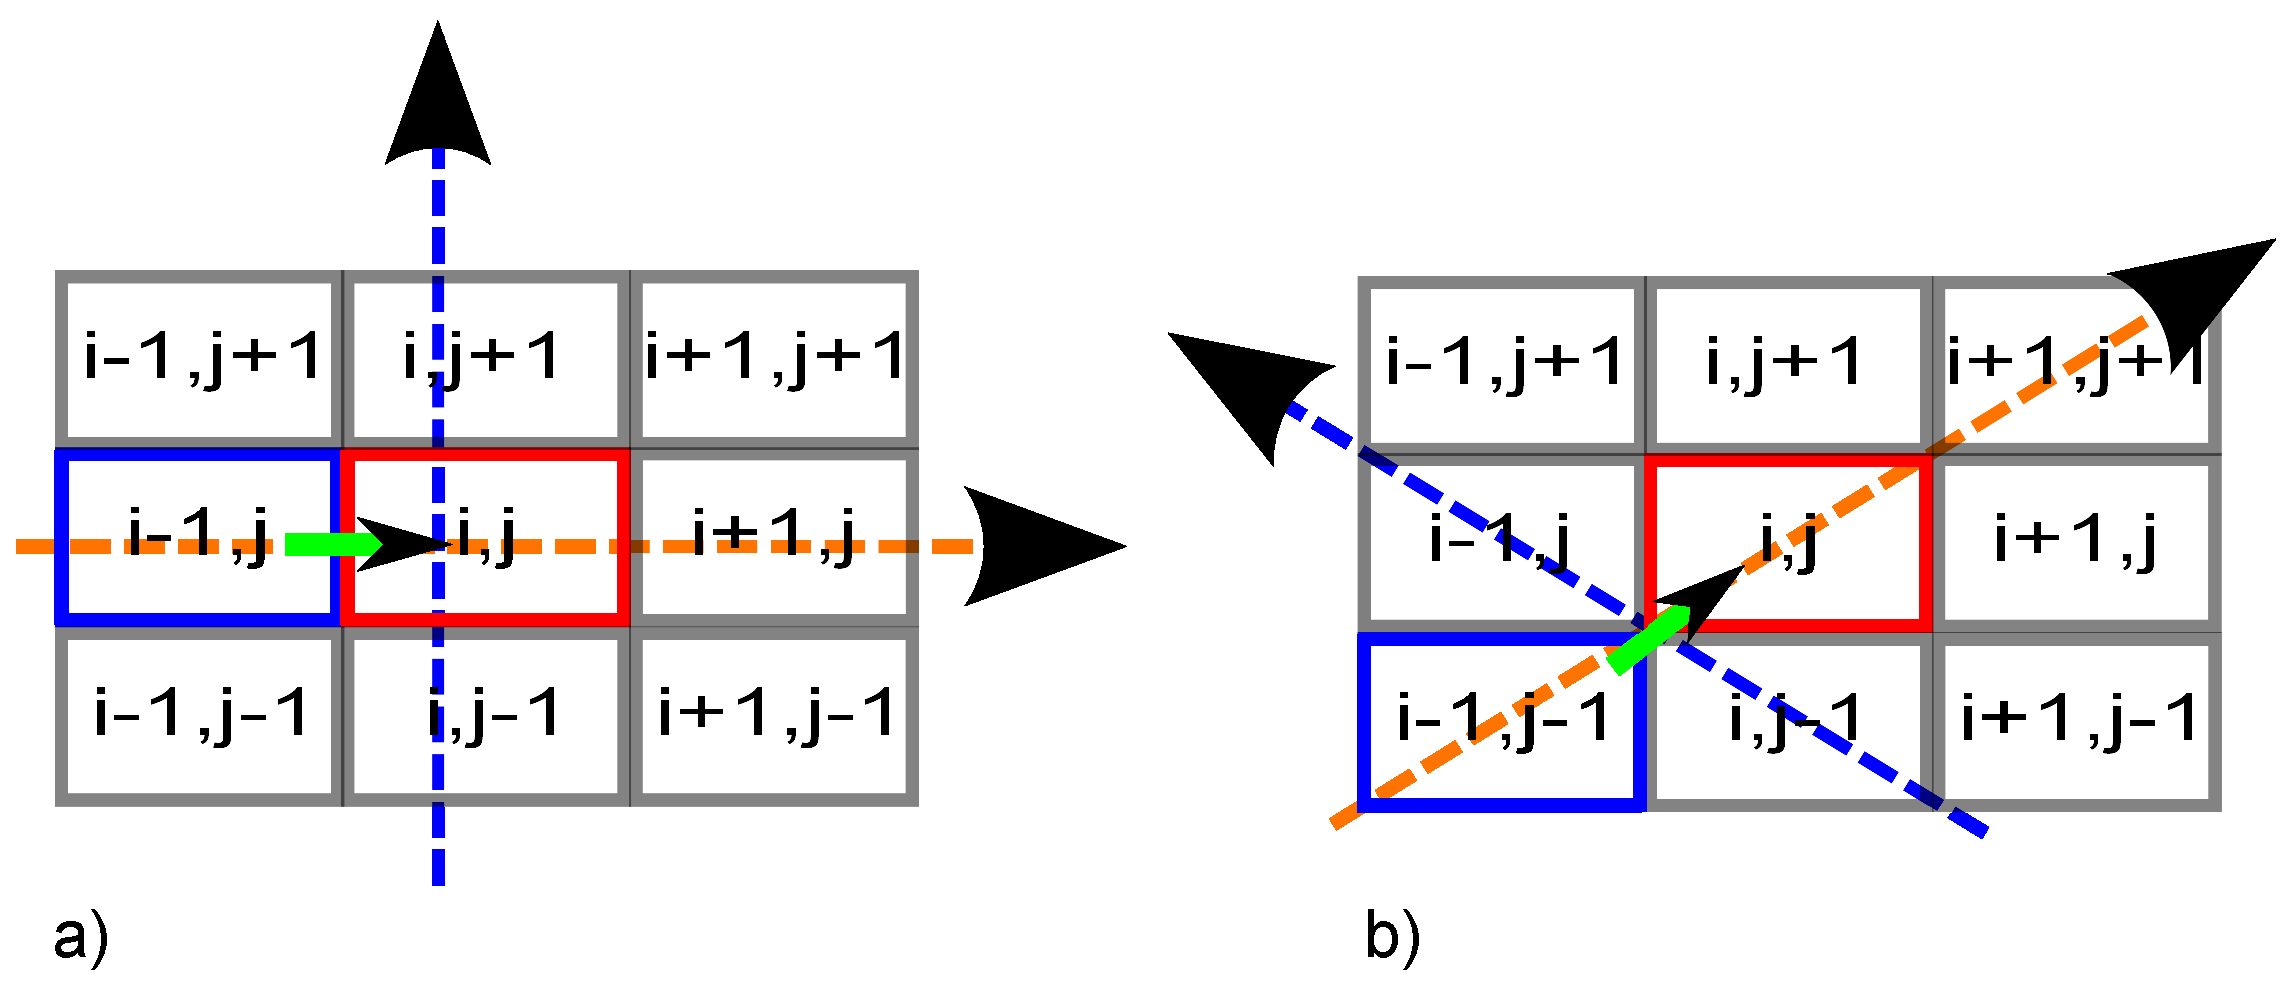
\includegraphics{axes.eps}}
\caption{The principal axis (in orange) and secondary axis (in blue) for two example movements. In a) the movement vector is horizontal, whereas in b) it is diagonal. The axes are not visually perpendicular in b) due to the fact that the cells are represented as rectangles rather than squares.}\label{fig:axes}
\end{figure*} 

\subsubsection{Active movement and proliferation}
In order to allow for condensation of mesenchyme around tips to occur, rules for movement and proliferation of mesenchymal cells are allowed. The probability of a move or proliferation occurring is assumed to depend on a cell's distance from the nearest epithelium cell. The pseudo-algorithm which is implemented is of the form:

\begin{enumerate}
\item Calculate the probability that a move/proliferation occurs. This is negatively related to the distance of each of the target cells to the nearest Ret-high epithelium.\label{point:mesactive}

\begin{equation}\label{eq:distance}
P(action) = \Phi(c_4 + c_5 \times distance)
\end{equation}

In (\ref{eq:distance}), $distance$ is the distance to the nearest Ret-high cell, and $c_5$ is chosen to be negative.

\item Draw a pseudo-random $X\sim unif(0,1)$. If $X<P(action)$ then proceed to the next step. If not, then proceed to the next cell in the randomised list of epithelium and mesenchyme created at the beginning of the update step.
\item Find all the possible targets for the mesenchyme cell from the 8-nearest-neighbours which are currently vacant. 
\item Select one from the set of targets probabilistically (using a multinomial logistic distribution), with targets further away from the epithelium penalised heavily in terms of their selection probability.\label{point:mesactive1}

\begin{equation} \label{eq:multilogit1}
P(target_j) = \frac{exp(c_6 + c_7\times distance_j)}{\sum\limits_{j} exp(c_6 + c_7\times distance_j)}
\end{equation}

In (\ref{eq:multilogit1}) $distance_j$ is the distance from the target cell to the nearest Ret-high cell.

\end{enumerate}

The epithelium is assumed to influence the movement of the mesenchyme in two ways. Firstly the probability that a move occurs inversely proportional to the distance of each potential target cell from the nearest Ret-high epithelium (see step \ref{point:mesactive}). The second mechanism directs the mesenchyme towards the nearest Ret-high epithelium (see step \ref{point:mesactive1}). This latter mechanism represents chemotaxis of mesenchyme towards the Ret-high epithelium. The choice to use the distance to the nearest Ret-high epithelium, rather than the epithelium in general, was chosen as to recreate the distinct lobes of mesenchyme seen \textit{in vivo}.

If chemotaxis occurs \textit{in natura} then it is likely driven by a chemoattractant which is produced by the epithelium, and diffuses in all directions. If the strength of the chemotactic force increases with the concentration of chemoattractant it is likely that the mesenchyme more distant from the epithelium will experience a weaker chemotactic force, and hence be less likely to move. However, if a move does occur the chemotaxis of the mesenchyme towards the epithelium would likely lead to a movement directed towards the epithelium. These aspects are implemented in rules \ref{point:mesactive} and \ref{point:mesactive1}.

We note that a particular form for the chemoattractant has not been proposed. Rather, it is proxied for, at each time step, by calculating a distance matrix which represents the distance of each point in the array from the nearest Ret-high epithelial cell. This calculation is done via dynamic programming for computational speed. The distance matrix is updated once per time step, as it is assumed that epithelium movements are not sufficiently significant to change qualitatively the movement of the mesenchyme within a cell cycle time.

\section{Parameter choice for quantitative results}\label{sec:parameters}
In section \ref{sec:quantresults}, the initial number of mesenchyme was varied in order to investigate its effect on the ultimate number of epithelium which make up the uretic bud. Here, parameter values were chosen as to represent a range which replicated the qualitative behaviour of the uretic bud. The parameter values chosen specifically were: $primary_{max} = 10$, $secondary_{max} = 10$ indicating the maximum distance a mesenchyme can be moved non-locally along the primary and secondary axes respectively. For Ret-low and Ret-high cells the values of $c_1$ and $c_2$ in (\ref{eq:probit}), were chosen to be (-150,50) and (-20,60) respectively. The dimensionless diffusion parameter $d_g$ was set to be 100.

\bibliographystyle{plain}
\bibliography{Kidney}


\end{document}
